% Generated by gen_figs.py from FROT tables/DRC_visualization_4.tex (program rules: benefit as % of PIA by claiming age).
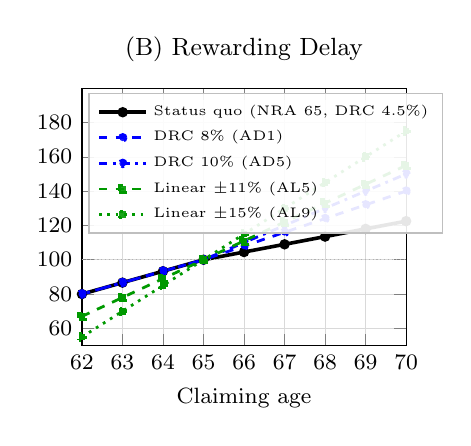
\begin{tikzpicture}
\begin{axis}[width=0.47\textwidth,height=0.40\textwidth,xmin=62,xmax=70,ymin=50,ymax=200,
  xtick={62,...,70},ytick={60,80,100,120,140,160,180},
  title={(B) Rewarding Delay},title style={font=\small},
  xlabel={Claiming age},
  grid=both,grid style={line width=.1pt, draw=gray!15},major grid style={line width=.2pt,draw=gray!30},
  tick label style={font=\footnotesize},label style={font=\footnotesize},
  legend style={font=\tiny,at={(0.02,0.98)},anchor=north west,draw=gray!50,fill=white,fill opacity=0.9,text opacity=1},legend cell align=left]
\addplot[black,line width=1.3pt,mark=*,mark size=1.2pt] coordinates {(62,80) (63,86.67) (64,93.33) (65,100) (66,104.5) (67,109) (68,113.5) (69,118) (70,122.5)};
\addlegendentry{Status quo (NRA 65, DRC 4.5\%)}
\addplot[blue,line width=1pt,dashed,mark=*,mark size=1.2pt] coordinates {(62,80) (63,86.67) (64,93.33) (65,100) (66,108) (67,116) (68,124) (69,132) (70,140)};
\addlegendentry{DRC 8\% (AD1)}
\addplot[blue,line width=1pt,dashdotted,mark=*,mark size=1.2pt] coordinates {(62,80) (63,86.67) (64,93.33) (65,100) (66,110) (67,120) (68,130) (69,140) (70,150)};
\addlegendentry{DRC 10\% (AD5)}
\addplot[green!60!black,line width=1pt,dashed,mark=square*,mark size=1.2pt] coordinates {(62,67) (63,78) (64,89) (65,100) (66,111) (67,122) (68,133) (69,144) (70,155)};
\addlegendentry{Linear $\pm$11\% (AL5)}
\addplot[green!60!black,line width=1pt,dotted,mark=square*,mark size=1.2pt] coordinates {(62,55) (63,70) (64,85) (65,100) (66,115) (67,130) (68,145) (69,160) (70,175)};
\addlegendentry{Linear $\pm$15\% (AL9)}
\draw[gray!60,densely dotted] (axis cs:62,100) -- (axis cs:70,100);
\end{axis}
\end{tikzpicture}
